% !TEX root = monografia.tex
\chapter{Aprendizado de Reforço}
\label{cap:reforco}

Aprendizado de Reforço é uma das grandes áreas que compõe Aprendizado de Máquina (?),
onde são estudados algoritmos que descrevem o comportamento de \textit{agentes} em um \textit{ambiente},
buscando o maior \textit{retorno} por suas ações.

\begin{figure}
    \centering
        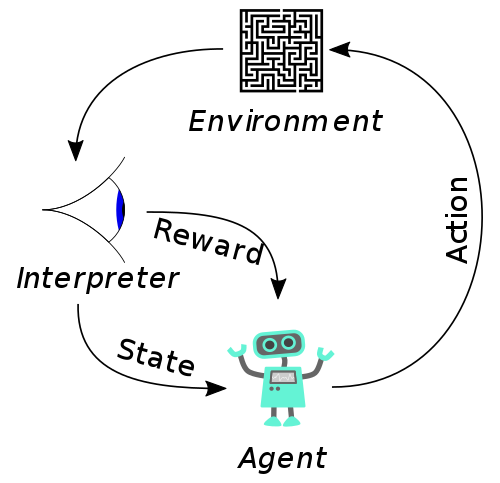
\includegraphics[width=5cm]{figuras/rl}
    \caption{Ilustração de Aprendizado de Reforço}
\end{figure}

Essa definição geral admite aplicação em uma grande quantidade de problemas (?),
sendo limitada principalmente pela existência de um ambiente que possa ser eficientemente simulado durante o processo de aprendizado do algoritmo.
Consequentemente, o aprendizado muitas vezes depende de uma quantidade grande de recursos computacionais.

Geralmente, os problemas da área são formulados como Processos de Decisão de Markov (MDP) finitos(?).
Um Processo de Decisão de Markov é uma quadrupla $(S,A,T,\gamma)$(?), onde:
\begin{itemize}
    \item $S$ é o conjunto de estados (que representa o ambiente)
    \item $A$ é o conjunto de ações que o agente pode tomar
    \item $T: S \times \mathbb{R} \times S \times A \to [0, 1]$ representa a probabilidade de um novo estado $s'$ e um retorno $r$ dados o estado atual $s$ e ação $a$
    \item $\gamma \in [0, 1]$ é um fator que determina o a importância de retornos futuros comparados com retornos imediatos.   
\end{itemize}

Em geral, o algoritmo não tem conhecimento algum das probabilidades de transição dos estados.

O agente interage com o ambiente gerando \textit{episódios}: 
$S_0, A_0, R_1, S_1, A_1, R_2, S_2, A_2, ..., R_T, \\S_T$.
Assim, o objetivo do agente é maximizar o \textit{retorno descontado} $G_1$ onde:
$G_t := R_t + \gamma R_{t + 1} + \gamma^2R_{t + 2} + ... = R_t + \gamma G_{t + 1}$.

Para isso, o agente define uma \textit{política} $\pi: A \times S \to [0, 1]$ 
que representa a distribuição de probabilidade da escolha das ações do agente em um dado estado $\pi(a | s)$.
Com isso em mãos podemos definir a função \textit{valor} de um estado $s$ na política $\pi$: $v_{\pi}(s) = \mathbb{E}_{\pi}[G_t | S_t = s]$ em um tempo $t$ qualquer.
E definimos também $q_{\pi}(s, a) = \mathbb{E}_{\pi}[G_t | S_t = s, A_t = a]$, a função \textit{ação-valor}.